\documentclass[11pt]{amsart}
\usepackage{geometry}  % See geometry.pdf to learn the layout options.
\geometry{letterpaper} % ... or a4paper or a5paper or ... 
\usepackage{graphicx}
\usepackage{amssymb}
\usepackage{epstopdf}
\DeclareGraphicsRule{.tif}{png}{.png}{`convert #1 `dirname #1`/`basename #1 .tif`.png}

\title{Final Report}
\author{Juan Durazo \\ Arthur Mitrano \\ Brendan Horan}
\date{May, 2013}  

\begin{document}

\maketitle

\section{Introduction}
\subsection{Problem} \indent \\
The problem we are seeking to solve is 
\begin{equation*}
  Ax=b, \indent A  \in  \mathbb{R}, \indent b = b^{exact} + b^{noise}.
\end{equation*}
In the above equation, $b^{noise}$ is a white noise vector with unknown level 
$\delta_{noise}$. We investigate how noise enters the problem through $b$ and 
how it propagates into the core problem. Using this information, we can develop
a stopping criteria for hybrid methods that are based on the Golub-Kahan 
bidiagonalization(GKb) process. Additionally, we can estimate the original noise
level that was introduced into the problem with $b$.

\section{Golub-Kahan iterative bidiagonalization}
Given the initial vector $w_{0}$ and $s_{1} = b/\beta_{1}$, where 
$\beta_{1} = \|b\| \neq 0$, the Golub-Kahan iterative bidiagonalization is
discribed by
\begin{align*}
  \alpha_{j}w_{j} &= A^{T}s_{j} - \beta_{j}w_{j-1}, &\quad \|w_{j}\|=1,\\
  \beta_{j+1}s_{j+1} &= Aw_{j} - \alpha_{j}s_{j}, &\quad \|s_{j+1}\|=1
\end{align*}
until $\alpha_{j} = 0$ or $\beta_{j+1} = 0$, or we reach the dimensionality of
the problem. Letting $S_{k} = [s_{1},\ldots,s_{k}]$ and 
$W_{k}= [w_{1},\ldots,w_{k}]$ be the left and right bidiagonalization matrices,
then:
\begin{equation*}
  A^{T}S_{k} = W_{k}L_{k}^{T}, \quad AW_{k} = [S_{k},s_{k+1}]L_{k+},
\end{equation*}
where
\begin{equation*}
  L_{k} =
  \begin{bmatrix}
    \alpha_{1} & & & \\
    \beta_{2} & \alpha_{2} & & \\
    & \ddots & \ddots & \\
    & & \beta_{k} & \alpha_{k}
  \end{bmatrix}, \quad
  L_{k+} = 
  \begin{bmatrix}
    L_{k} \\
    \beta_{k+1}e_{k}^{T}
  \end{bmatrix}
\end{equation*}
Since this process leads to orthogonal matrices $S_{k}$ and $W_{k}$, we can
calculate the singular value decomposition of A as $A = S_{k}L_{k}W_{k}^{T}$
$= S_{k}U\Sigma V^{T}W_{k}^{T} = U_{k}\Sigma V_{k}^{T}$, with $U_{k}$ and 
$V_{k}$ orthogonal, since product of orthogonal matrices are orthogonal. This is
a stable way to calculate the SVD of $A$ \cite{svdRef}.

The GKIB applied on the problem $Ax = b$ is closely related to the
\emph{Lanczos tridiagonalization} of the matrix $AA^{T}$ with starting vector
$s_{1} = b/\beta_{1}$, $\beta_{1} = \|b\|$, yielding after $k$ steps:
\begin{equation} \label{eq:tridiag}
  AA^{T}S_{k} = S_{k}T_{k} + \alpha_{k}\beta_{k+1}s_{k+1}e_{k}^{T},
\end{equation}
with
\begin{equation*}
  T_{k} = L_{k}L_{k}^{T} = 
  \begin{bmatrix}
    \alpha_{1}^{2} & \alpha_{1}\beta_{2} & & \\
    \alpha_{1}\beta_{2} & \alpha_{2}^{2} + \beta_{2}^{2} & \ddots & \\
    & \ddots & \ddots & \alpha_{k-1}\beta_{k} \\
    & & \alpha_{k-1}\beta_{k} & \alpha_{k}^{2} + \beta_{k}^{2}
  \end{bmatrix}
\end{equation*}
The matrix $L_{k}$ is a Cholesky factor of the matrix $T_{k}$.
% Maybe we should add here information about the Ritz values or move this to a
% different section.

If we look for solutions of the original problem $Ax \approx b$ on the range of
$W_{k}$, i.~e.~, considering $x_{k} = W_{k}y_{k}$ as such solution, the residual
can be expressed as
\begin{align*}
  r_{k} = b - AW_{k}y_{k} &= S_{k+1}(\beta_{1}e_{1} - L_{k+}y_{k}) \\
  &= S_{k}(\beta_{1}e_{1} - L_{k}y_{k}) - 
  (\beta_{k+1}e_{k}^{T}y_{k})s_{k+1},
\end{align*}.
Using the orthogonality of $s_{k}$'s and the residual expression, we get two 
classes of subproblems:
\begin{enumerate}
  \item If we require that the residual $r_{k}$ to be orthogonal to $S_{k}$:
    \begin{equation*}
      L_{k}y_{k} = \beta_{1}e_{1}, \quad L_{k} \in \mathbb{R}^{k \times k},
    \end{equation*}
    which corresponds to the CGME(?) method.
  \item If we minimize the norm of the residual we get
    \begin{equation*}
      y_{k} = argmin_{y}\|L_{k+}y - \beta_{1}e_{1}\|
    \end{equation*}
    which corresponds to CGLS or LSQR method.
\end{enumerate}
For both kinds of subproblems the information used depends on the vector $b$ and
the bidiagonal matrix ($L_{k}$ or $L_{k+}$), this often refer as the core or
projected problem. The bidiagonalization concentrates the useful information of
the main problem on its bidiagonal block. In presence of noise, those
subproblems might be polluted by it. A better understanding on how this noise
propagates through the GKIB may aid on solving the ill-posed problem.

\section{Test problem: Shaw}
Most of the numerical experiments presented in this report are based on the 
problem \texttt{shaw(400)} from the Regularization Toolbox \cite{hansen}. $A$,
$b^{exact}$ and the exact solution $x$ are created by 
\texttt{[A, b\_exact, x] = shaw(400)}. Noise is added ($b^{noise}$) using the
Matlab \texttt{rand(400,1)}, which is scaled such that
\begin{equation*}
  \delta_{\text{noise}} = \frac{\|b^{\text{noise}}\|}{\|b^{\text{exact}}\|}.
\end{equation*}
We used $\delta_{\text{noise}} = 10^{-14}, 10^{-8}, 10^{-4}$ as noise level.
The shaw problem satisfy the \emph{discrete Picard condition} on average 
(without added noise). On figure \ref{fig:picard} we see that the Picard 
condition is drastically violated due to the complete dominance of the noise in
the projections of $b$ onto the left singular vectors $u_{j}$ of $A$.
\begin{figure}[htb] \label{fig:picard}
  \begin{center}
    %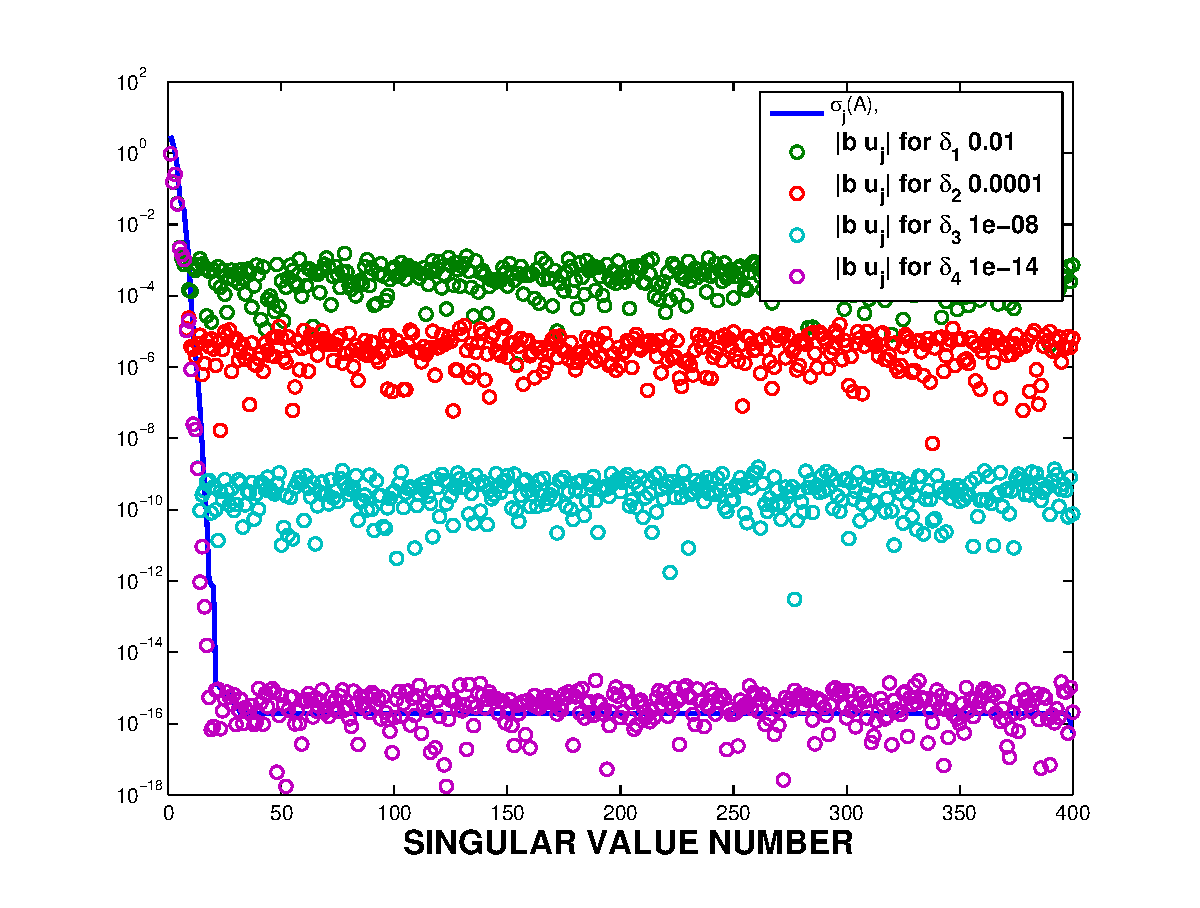
\includegraphics[width=.55\linewidth]{figures/picard}
  \end{center}
\caption{Singular values $\sigma_{j}$ and the absolute value of the
projections of the noisy right-hand side $b$ on the left singular vectors 
$u_{j}$ of $A$. $\delta_{\text{noise}} = 10^{-14}, 10^{-8}, 10^{-4}$.}
\end{figure}
If one can check that the discrete Picard condition holds for the shaw problem
using high precision arithmetic.
% We could include the vpa plot for completeness.

\section{Analyzing the spectral coefficients of $s_{k}$}
Now we focus our attention on studying and interpreting the spectral 
coefficients of the vectors $s_{k}$'s. This will give the information on how the
noise spreads on the problem solution.

The singular vectors $u_{k}$'s increase in frequency as $k$ increase, see figure
\ref{fig:singularVectors}. In figure \ref{fig:spectralCoeffs} we see that as $k$
is increased the spectral coefficients associated with the lower frequencies 
singular vectors decay and the ones associated with the high frequencies rise 
until they are comparable. This behavior is consider to reveal the noise.
\begin{figure}[htb] \label{fig:singularVectors}
  \begin{center}
    %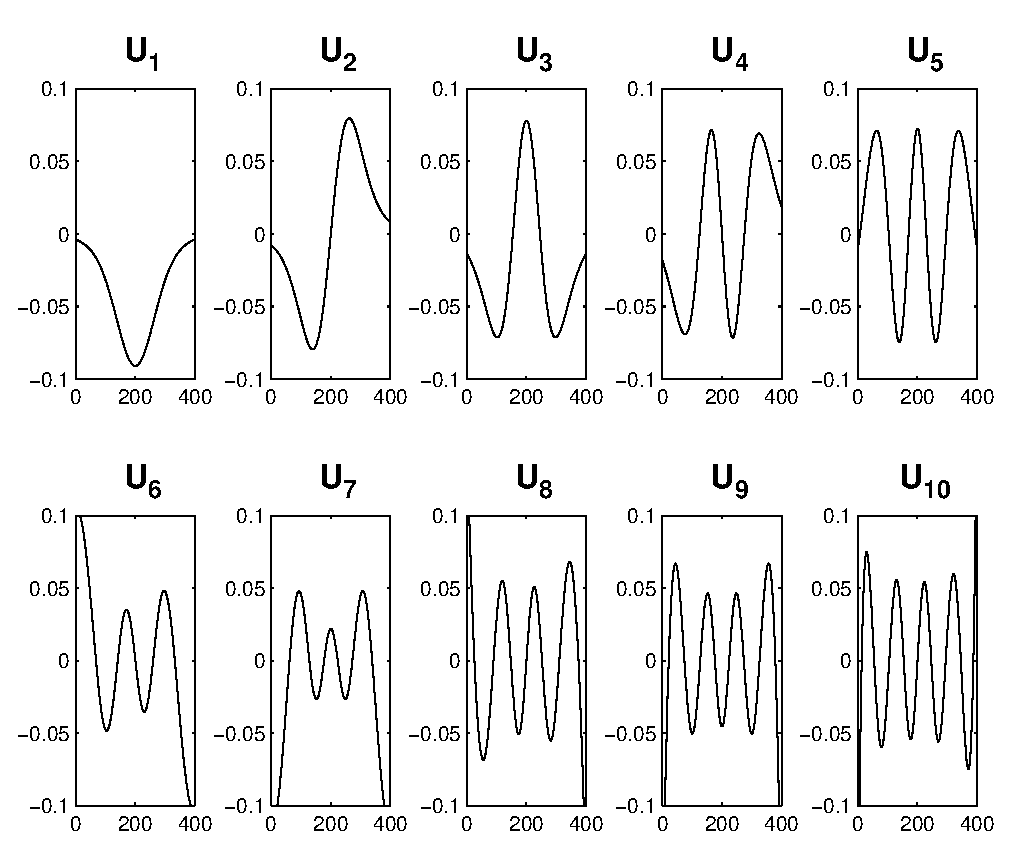
\includegraphics[width=0.55\linewidth]{figures/run1/sing_vecs}
  \end{center}
\caption{Note that the frequency of the singular vector increase with $k$.}
\end{figure}
\begin{figure}[htb] \label{fig:spectralCoeffs}
  \begin{center}
    %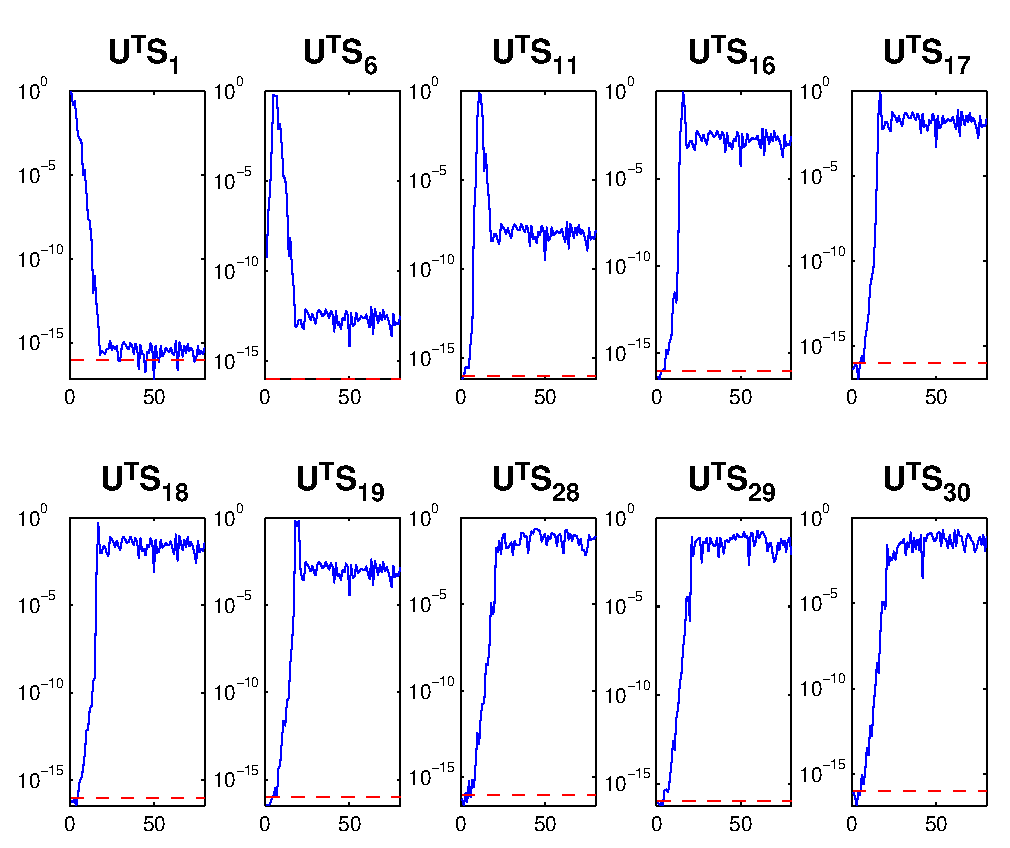
\includegraphics[width=0.55\linewidth]{figures/run1/spec_sk}
  \end{center}
\caption{Plot of the first 80 spectral coefficients on the direction of the left
singular vectors of $A$. As $k$ increases the lower frequencies get filtered out
and the high frequencies become comparable.}
\end{figure}

To better see what is happening we can use the singular value decomposition of
$A$ and the Lanczos tridiagonalization \eqref{eq:tridiag} of $AA^{T}$ to deduce
\begin{equation} \label{eq:spectralCoeffs}
  \Sigma^{2}(U^{T}S_{k}) = (U^{T}S_{k})(L_{k}L_{k}^{T}) + 
  \alpha_{k}\beta_{k+1}(U^{T}s_{k+1})e_{k}^{T}.
\end{equation}
Setting $k = 1$ we can see how the noise spreads from $s_{1}$ to $s_{2}$,
looking to the last column of \eqref{eq:spectralCoeffs} we get:
\begin{equation*}
  \alpha_{1}\beta_{2}(U^{T}s_{2}) = (\Sigma^{2} - \alpha_{1}^{2}I)U^{T}s_{1}.
\end{equation*}
So the spectral coefficients of $s_{2}$ are multiplied by
\begin{equation*}
  \frac{\sigma_{k}}{\alpha_{1}\beta_{2}} - \frac{\alpha_{1}}{\beta_{2}},
\end{equation*}
where the constant $\alpha_{1}/\beta_{2}$ is likely larger than 1. Hence, for 
$k$ small we are multiplying by smaller number, and for large $k$ values the
singular values $\sigma_{k}$ are negligible, which makes the spectral
coefficients associated amplified ($\alpha_{1}/\beta_{2}$) see section 3.1 of 
\cite{bidiagonalization} and figure \ref{fig:rhok}.



\section{Finding $\bf k_{noise}$ using Normalized Cumulative Periododogram}
The Normalized Cumulative Periodogram(NCP) can be used to determine how 
"white-noise like" each $s_k$ is.

\begin{thebibliography}{1}
  \bibitem{bidiagonalization}  Hnetynkova, I. and Plesinger, M.. 
    \emph{The regularizing effect of the Golub-Kahan iterative bidiagonalization 
      and revealing the noise level in the data.}
      BIT Numer Math (2009) 49: 669-696.
    \bibitem{hansen} [17] Ivete
\end{thebibliography}

\end{document}  
